The aim of this procedure, proposed by Vamvatsikos (2014), is the estimation of the median spectral acceleration value $\hat{S}_{a,ds}$, that brings the structure to the attainment of a set of damage states \textit{ds}, and the corresponding dispersion beta $\beta_{S_a}$, the parameters needed for the mathematical representation of fragility in equation \ref{eq:fragility-definition}. The aim is achieved making use of the work by Ruiz-Garcia and Miranda (2007), where the inelastic displacement demand of bilinear SDoF systems is related to the elastic displacement with a simple relationship.

The C$_R$-based procedure presented herein is applicable to bilinear elasto-plastic capacity curve only, and it is suitable for single building fragility curve estimation, as described in section \ref{subsubsec:single-building}. However the fragility curves derived for single buildings can be combined in a unique fragility curve, which considers also the inter-building uncertainty, as described in the following sections.

\subsubsection{Single Building Fragility and Vulnerability function}
\label{subsubsec:single-building}
This procedure provides a simple relationship between median damage state threshold, expressed in terms of top displacement $\hat{d}_{roof, ds}$, at each damage state threshold \textit{ds}, and the corresponding median elastic Spectral displacement value $\hat{S}_{d,ds}(T_1)$.

\begin{equation}
\hat{d}_{roof, ds} = C_R \hat{S}_{d, ds}(T_1) \Gamma_1 \Phi_1
\end{equation}

where $\Gamma_1 \Phi_1$ is the first mode participation factor estimated for the first-mode shape normalised by the roof displacement, and C$_R$ is the inelastic displacement ratio (inelastic over elastic spectral displacement), computed by Ruiz-Garcia and Miranda (2007) for nonlinear SDoF systems, which is a function of the first-mode period of vibration and the relative lateral strength of the system R. Therefore the median Spectral acceleration at the fundamental period of vibration $\hat{S}_{a,ds}(T_1)$ turns out to be expressed as a function of the roof displacement according to the following equation:

\begin{equation}
\hat{S}_{a,ds}(T_1) = \frac{4 \pi^2}{\hat{C}_R T^2 \Gamma_1 \Phi_1} \hat{d}_{roof, ds}
\label{eq:Sa_RGM}
\end{equation}

Estimates of $\hat{C}_R$ parameter are provided by Ruiz-Garcia and Miranda (2007), as result of nonlinear regression analysis of three different measures of central tendency computed from 240 ground motions:

\begin{equation}
\hat{C}_R = 1 + \frac{\hat{R} - 1}{79.12 T_1 ^{1.98}}
\label{eq:Cr_RGM}
\end{equation}

where $\hat{R}$ is given by the following equation:

\begin{equation}
\hat{R}_{ds} = max(0.425(1 - c + \sqrt{c^2 + 2c(2 \hat{\mu}_{ds} - 1) + 1}),1)
\label{eq:R_RGM}
\end{equation}

where c = 79.12 T$^{1.98}$, and $\hat{\mu}_{ds}$ is the median ductility level at the damage state threshold of interest.

For what concerns $\beta_{S_a}$, the dispersion of $\hat{S}_{a,ds}$, it can be computed either in a simplified way or with a comprehensive procedure.

In the simplified approach the following relationship between $S_a$ and the median EDP damage threshold $\hat{\theta}$ (Cornell, 2002) is used:

\begin{equation}
\hat{\theta} = a S_a^b
\end{equation}

so that $\beta_{S_a}$ can be easily derived from the dispersion of $\theta$ due to record-to-record variability, $\beta_{\theta d}$, as in the following:

\begin{equation}
\beta_{S_a} = \frac{1}{b} \beta_{\theta d}
\label{eq:betaSa_RGM}
\end{equation}

$\beta_{\theta d}$ can be obtained assuming that top drift $d_{roof}$ and $\theta$ are proportional, and they thus share the same dispersion. Moreover the dispersion of $d_{roof}$ is the same as the dispersion of C$_R$, since they are also proportional. Finally $\beta_{\theta d}$ can be computed with the following equation, which represents Ruiz-Garcia and Miranda's (2007) estimate of C$_R$ dispersion:

\begin{equation}
\sigma_{\ln(C_R)} = \sigma_{\ln(d_{roof})} = \beta_{\theta d} =  1.975 [\frac{1}{5.876} + \frac{1}{11.749 (T + 0.1)}] [1- \exp(-0.739 (R - 1))]
\label{eq:beta_eq_RGM}
\end{equation}

Uncertainty in the damage state can also be accounted for combining the dispersion of $\theta$ due to uncertainty in the damage state with the dispersion due to record-to-record variability, as in the following equation:

\begin{equation}
\beta_{S_a} = \frac{1}{b} \sqrt{\beta_{\theta d}^2 + \beta_{\theta c}^2}
\label{eq:betaStot_RGM}
\end{equation}

In the comprehensive approach the relationship between the 16$^{th}$, 50$^{th}$ and 84$^{th}$ fractiles of $\mu$ and R needs to be drawn, as represented in Figure \ref{fig:Rmu}. This is done by computing $\beta_{\theta d}$ for a discretised number of R with eq. \ref{eq:beta_eq_RGM}, and obtaining from this value the 16$^{th}$ and 84$^{th}$ fractiles of $\mu$ ($\mu_{16\%}$ and $\mu_{84\%}$), according to the Equations \ref{eq:mu16-beta} and \ref{eq:mu84-beta}.

\begin{figure}[!htbp]
\centering
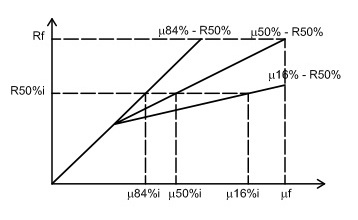
\includegraphics[width=8cm]{./figures/Rmu.jpg}
\caption{R-$\mu$ relationship.}
\label{fig:Rmu}
\end{figure}

\begin{equation}
\mu_{ds,16} = \hat{\mu}_{ds} e^{-\beta_{\theta d,ds}}
\label{eq:mu16-beta}
\end{equation}
\begin{equation}
\mu_{ds,84} = \hat{\mu}_{ds} e^{\beta_{\theta d,ds}}
\label{eq:mu84-beta}
\end{equation}

The median $R_{50\%}$ values have been already computed with eq. \ref{eq:R_RGM}, and $\mu_{16\%}$-$R_{50\%}$, $\mu_{50\%}$-$R_{50\%}$ and $\mu_{84\%}$-$R_{50\%}$ curves can now be drawn.
If uncertainty in the damage criteria $\beta_{\theta c}$ is equal to 0 the $R_{50\%}$, $R_{16\%}$, and $R_{84\%}$ values corresponding to the ductility limit states $\mu_{ds}$ are found interpolating the aforementioned R-$\mu$ curves, and converted into $\hat{S}_{a,ds}$ and $\beta_{S_{a d}}$ according to the following equations:

\begin{equation}
\hat{S}_{a,ds} = R_{50\%}(\mu_{ds}) S_{ay}
\label{eq:SaR}
\end{equation}
\begin{equation}
\beta_{S_{a d}} = \beta_{R(\mu)} = \frac{\ln R(\mu)_{84\%} - \ln R(\mu)_{16\%}}{2}
\label{eq:betaR}
\end{equation} 

where
\begin{equation}
S_{ay} = \frac{4 \pi^2 d_{roof,y}}{T_1^2 g \Gamma_1}
\label{eq:Say}
\end{equation}

If $\beta_{\theta c}$ is different from 0 instead, different values of ductility limit state are sampled from the lognormal distribution with median the median value of the ductility limit state, and dispersion the input $\beta_{\theta c}$.
For each of these ductilities the corresponding $R_{50\%}$, $R_{16\%}$, and $R_{84\%}$ values are found interpolating the aforementioned curves, and converted into $\hat{S}_{a,ds}$ and $\beta_{S_{a d}}$ according to Equations \ref{eq:SaR} and \ref{eq:betaR}.

MC random S$_a$ for each of the MC sampled ductility limit states are computed using $\hat{S}_{a,ds}$ and $\beta_{S_{a d}}$, and their median and dispersion are estimated. These parameters constitute the median $\hat{S}_{a,ds}$ and the total dispersion $\beta_{S_a}$ for the considered damage state. The procedure is repeated for each damage state.

To derive a discrete vulnerability function at certain intensity measure levels, the input damage-to-loss factors are applied to the probability of occurance of each damage state, extracted from the probability of exceedance of each damage state described by the fragility function.
If dispersion due to uncertainty in the limit state is different from zero a vulnerability function is derived for the MC sets of sampled ductility limit states. It results in MC loss ratios (LRs) for each defined intensity measure levels. Finally a lognormal distribution of the loss ratios is assumed at each iml with mean and standard deviation the mean and standard deviation of the all the computed LRs.

\subsubsection{Multiple-Building Fragility and Vulnerability function}
\label{subsubsec:multiple-buildings}
If multiple buildings have been input to derive fragility function for a class of buildings all $\hat{S}_{a, blg}$ and $\beta_{S_a, blg}$ are combined in a single lognormal curve. A minimum of 5 buildings should be considered to obtain reliable results for the class.\\ 
A new issue arises when multiple buildings are considered: the S$_a$ at the fundamental period of each building should be converted to a common intensity measure, to be able to combine the different fragility functions. A common intensity measure is selected to be S$_a$ at the period T$_{av}$, which is a weighted average of the individual building fundamental periods T$_1$. Then each individual fragility needs to be expressed in terms of the common S$_a$(T$_{av}$), using a spectrum. FEMA P-695 far field set of 44 accelerograms (22 records for the two directions) was used to derive a mean uniform hazard spectrum, and the ratio between the S$_a$ at different periods is used to scale the fragility functions. It can be noted that the actual values of the spectrum are not important, but just the spectral shape. 
The median $\hat{S}_a$ is converted to the mean $\mu_{ln(S_a)}$ of the corresponding normal distribution ($\mu_{ln(S_a)} = ln(\hat{S}_a)$) and, simply scaled to the common intensity measure as follows:

\begin{equation}
\mu_{ln(S_a), blg} = \mu_{ln(S_a), blg} S(T_{av})/ S(T_{1, blg})
\end{equation}
\begin{equation}
\beta_{S_a, blg} = \beta_{S_a, blg} S(T_{av})/ S(T_{1, blg})
\label{eq:Sa(Tav)}
\end{equation}

Finally the parameters of the single lognormal curve for the class of buildings, mean and dispersion, can be computed as the weighted mean of the single means and the weighted SRSS of the inter-building and intra-building standard deviation, the standard deviation of the single means and the single dispersions respectively, as shown in the following equations:

\begin{equation}
\mu_{ln(S_a), tot} = \sum_{i=0}^{n.blg} w_{blg-i} \mu_{ln(S_a), blg-i}
\label{eq:combination-lognormals-mu}
\end{equation}
\begin{equation}
\beta_{S_a, tot} = \sqrt{ \sum_{i=0}^{n.blg} w_{blg-i} ((\mu_{ln(S_a), blg-i}-\mu_{ln(S_a), tot})^2+ \beta_{S_a, blg-i}^2})
\label{eq:combination-lognormals-sigma}
\end{equation}

The mean $\mu_{ln(S_a)}$ and total dispersion $\beta_{S_a}$ of the fragility function of the class are converted to logarithmic mean $\mu_{S_a}$ and logarithmic covariance $cov_{S_a}$ (standard deviation $\sigma_{S_a}$ over $\mu_{S_a}$), according to the following equations:

\begin{equation}
\hat{S}_a = e^{\mu_{ln(S_a)}}
\end{equation}
\begin{equation}
\mu_{S_a} = \hat{S}_a e^{\frac{\beta_{S_a}^2}{2}}
\label{eq:median-to-mean}
\end{equation}
\begin{equation}
\sigma_{S_a} = \sqrt[2]{(\beta_{S_a}^2-1) e^{2\ln{ \hat{S}_a}+\beta_{S_a}^2}}
\label{eq:dispersion-to-standard}
\end{equation}
\begin{equation}
cov_{S_a} = \frac{\sigma_{S_a}}{\mu_{S_a} }
\end{equation}

A vulnerability function for a class of buildings can also be obtained, from the single building vulnerability functions. The input damage-to-loss function is applied to the fragility function derived for each building. For the selected intensity measure levels a value of loss ratio $LR_{blg}$ is thus defined for each building. A discrete vulnerability function for the entire class of buildings is represented at each iml by a mean LR, $\mu_{LR,tot}$, equal tot the weighted $LR_{blg}$, and a standard deviation, $\sigma_{LR, tot}$, equal to the weighted standard deviation of all the computed $LR_{blg}$. The $\sigma_{LR, tot}$ of the fragility function of the class is converted to covariance $cov_{LR}$ (standard deviation $\sigma_{LR, tot}$ over $\mu_{LR, tot}$).

\subsubsection{Inputs}
\label{subsubsec:InputCr}
The inputs must be formatted as comma-separated value files (.csv), and saved in the folder \textit{input}, contained in the NSP directory. If any other environment different from Windows is used make sure that the "comma separated values Windows" is selected as saving option when creating the input files. 

If multiple buildings want to be analysed to consider the inter-building uncertainty the parameters relative to each building should be added as additional lines in the input tables, as shown in the examples below, otherwise a single line must be input.

If the user has at disposal an idealised elasto-plastic pushover curve for each building, that is to say that the variable \textit{in\_type} has been set to 0, the following data need to be provided in the corresponding csv files:

\begin{enumerate}
\item First period of vibration T$_1$, corresponding modal participation factor $\Gamma_1$, normalised with respect to the roof displacement, and weight for the combination of different buildings, input in \textit{building\_parameters.csv}, as in the example below:
	\begin{table}[!htbp]
	\centering
	\begin{tabular}{|c|c|c|c|} \hline
	\textbf{n.building} & \textbf{T$_1$} & \textbf{$\Gamma_1$} & \textbf{weights}\\ \hline
	1 & 0.32 & 1.23 & 0.2\\ \hline
	2 & 0.40 & 1.25 & 0.3\\ \hline
	... & ... & ... & ... \\ \hline
	\end{tabular}
	\end{table}
	
\item Roof displacement at each limit state LS and corresponding dispersion $\beta_{\theta c}$ input in \textit{displacement\_profile.csv}, as shown in the example below. If dispersion is unknown, $\beta_{\theta c}$ can be set equal to zero at each LS.
	\begin{table}[!htbp]
	\centering
	\begin{tabular}{|c|c|c|c|} \hline
	\textbf{n.building} & \textbf{LS$_1$} &	\textbf{LS$_2$} &	\textbf{LS$_3$} \\ \hline
	1 & 0.066 & 0.169 & 0.23\\ \hline
	$\beta_{\theta d, 1}$ & 0.1 & 0.3 & 0.4\\ \hline
	2 & 0.08 & 0.172 & 0.25\\ \hline
	$\beta_{\theta d, 2}$ & 0.1 & 0.3 & 0.4\\ \hline	
	\end{tabular}
	\end{table}
	
\item Idealised pushover curve, input in \textit{idealised\_curve.csv} as shown below. The only required parameters are the yielding displacement $d_y$, the ultimate displacement $d_u$ and the yielding force F$_y$.

\begin{table}[!htbp]
\centering
\begin{tabular}{|c|c|c|c|} \hline
\textbf{n.building} & \textbf{d$_y$} & \textbf{d$_u$} & \textbf{F$_y$} \\ \hline
1 & 0.09	& 0.3	 & 523\\ \hline
2 & 0.12	& 0.35	 & 400\\ \hline
... & ...	& ... & ...\\ \hline
\end{tabular}
\end{table}

\item Consequence model (loss ratio per each damage state) consistent with the defined set of damage states, input in \textit{consequence.csv}, as in the example below. A single consequence model can be input. This input is needed only if the variable \textit{vuln} has been set to 1.	
	\begin{table}[!htbp]
	\centering
	\begin{tabular}{|c|c|c|} \hline
	\textbf{DS$_1$} & \textbf{DS$_2$} & \textbf{DS$_3$} \\ \hline
	0.2	& 0.5	 & 1\\ \hline
	\end{tabular}
	\end{table}
	
\end{enumerate}

The user can also decide to input displacements vs base shear at each time step results from a pushover analysis, setting the variable \textit{in\_type} = 0 in the option section. The aforementioned inputs can be used either to derive multilinear idealised curves, setting the option \textit{idealised} = 0, or just to convert the limit states from drift values to roof displacement values without assumptions, and still input an idealised curve, setting the option \textit{idealised} = 1. The following data need to be provided in the corresponding csv files:

\begin{enumerate}
\item T$_1$ and corresponding $\Gamma_1$, weight for the combination of different buildings, number of storeys and height of each storey, input in \textit{building\_parameters.csv}, as in the example below:
	\begin{table}[!htbp]
	\centering
	\begin{tabular}{|c|c|c|c|c|c|c|c|c|} \hline
	\textbf{n.building} & \textbf{T$_1$} & \textbf{$\Gamma_1$} & \textbf{weights} & \textbf{n.Storey} & \textbf{H$_1$} & \textbf{H$_2$} & ... & \textbf{H$_n$} \\ \hline
	1 & 0.32 & 1.23 & 0.2 & 4 & 3 & 3 & ... & 3 \\ \hline
	2 & 0.40 & 1.25 & 0.3 & 4 & 4 & 2.7 & ... & 2.7 \\ \hline
	... & ... & ... & ... & ... & ... & ... & ... & ... \\ \hline
	\end{tabular}
	\end{table}
	
\item Displacements at each storey, at each incremental step of the pushover analysis, input in \textit{displacements\_pushover.csv}, as in the example below: 
	\begin{table}[!htbp]
	\centering
	\begin{tabular}{|c|c|c|c|c|c|c|} \hline
	\textbf{n.building} & \textbf{n.Storey} & \textbf{Step1} & \textbf{Step 2} & \textbf{Storey 3} & ... & \textbf{Step n}\\ \hline
	1 &	1 & 0.0001 &	0.0005 &	0.001 & ... & 0.01\\ \hline
	   &	2 & 0.0003 &	0.0010 &	0.002 & ... & 0.02\\ \hline
	   &	3 & 0.0004 &	0.0016 &	0.003 & ... & 0.03\\ \hline
	   &	4 & 0.0006 &	0.0021 &	0.004 & ... & 0.04\\ \hline
	2 &	1 & 0.0001 &	0.0005 &	0.001 & ... & 0.01\\ \hline
	   &	2 & 0.0005 &	0.0012 &	0.002 & ... & 0.03\\ \hline
	   &	... & ... &	... &	... & ... & ...\\ \hline
	\end{tabular}
	\end{table}
	
\item Base shear at each incremental step of the pushover analysis input in \textit{reactions\_pushover.csv}, as in the example below:
	\begin{table}[!htbp]
	\centering
	\begin{tabular}{|c|c|c|c|c|c|} \hline
	\textbf{n.building} &	\textbf{Step1} & \textbf{Step 2} & \textbf{Storey 3} & ... & \textbf{Step n} \\ \hline
	1 & 0.35 & 0.69 & 1.04 & ... & 29.12\\ \hline
	2 & 0.45 & 0.78 & 2.05 & ... & 40.00\\ \hline
	... & ... & ... & ... & ... & ...\\ \hline
	\end{tabular}
	\end{table}
	
\item Drift limit state and corresponding dispersion $\beta_{\theta c}$ input in \textit{limits.csv}. If dispersion is unknown, $\beta_{\theta c}$ can be set equal to zero at each limit state.
	\begin{table}[!htbp]
	\centering
	\begin{tabular}{|c|c|c|c|} \hline
	\textbf{n.building} & \textbf{LS$_1$} &	\textbf{LS$_2$} &	\textbf{LS$_3$} \\ \hline
	1 & 0.01 &	0.025 & 0.0337\\ \hline
	$\beta_{\theta d, 1}$ &	0.1 & 0.2 & 0.25\\ \hline
	2 & 0.014 &	0.030 & 0.0430\\ \hline
	$\beta_{\theta d, 2}$ &	0.1 & 0.2 & 0.25\\ \hline
	\end{tabular}
	\end{table}

\item Idealised pushover curve, input in \textit{idealised\_curve.csv} if the option \textit{idealised} = 1, as shown below. 
\begin{table}[!htbp]
\centering
\begin{tabular}{|c|c|c|c|} \hline
\textbf{n.building} & \textbf{d$_y$} & \textbf{d$_u$} & \textbf{F$_y$} \\ \hline
1 & 0.09	& 0.3	 & 523\\ \hline
2 & 0.12	& 0.35	 & 400\\ \hline
... & ...	& ... & ...\\ \hline
\end{tabular}
\end{table}

\item Consequence model (loss ratio per each damage state) consistent with the defined set of damage states, input in \textit{consequence.csv}, as in the example below. A single consequence model can be input. This input is needed only if the variable \textit{vuln} has been set to 1.
	\begin{table}[!htbp]
	\centering
	\begin{tabular}{|c|c|c|} \hline
	\textbf{DS$_1$} & \textbf{DS$_2$} & \textbf{DS$_3$} \\ \hline
	0.2	& 0.5	 & 1\\ \hline
	\end{tabular}
	\end{table}
	
\end{enumerate}

\subsubsection{Calculation Steps}
The overall workflow of C$_R$-based procedure is summarised in this section and represented in Figure \ref{fig:Cr_workflow} for the case of a single building fragility/vulnerability function. 

\begin{figure}[!htbp]
\centering
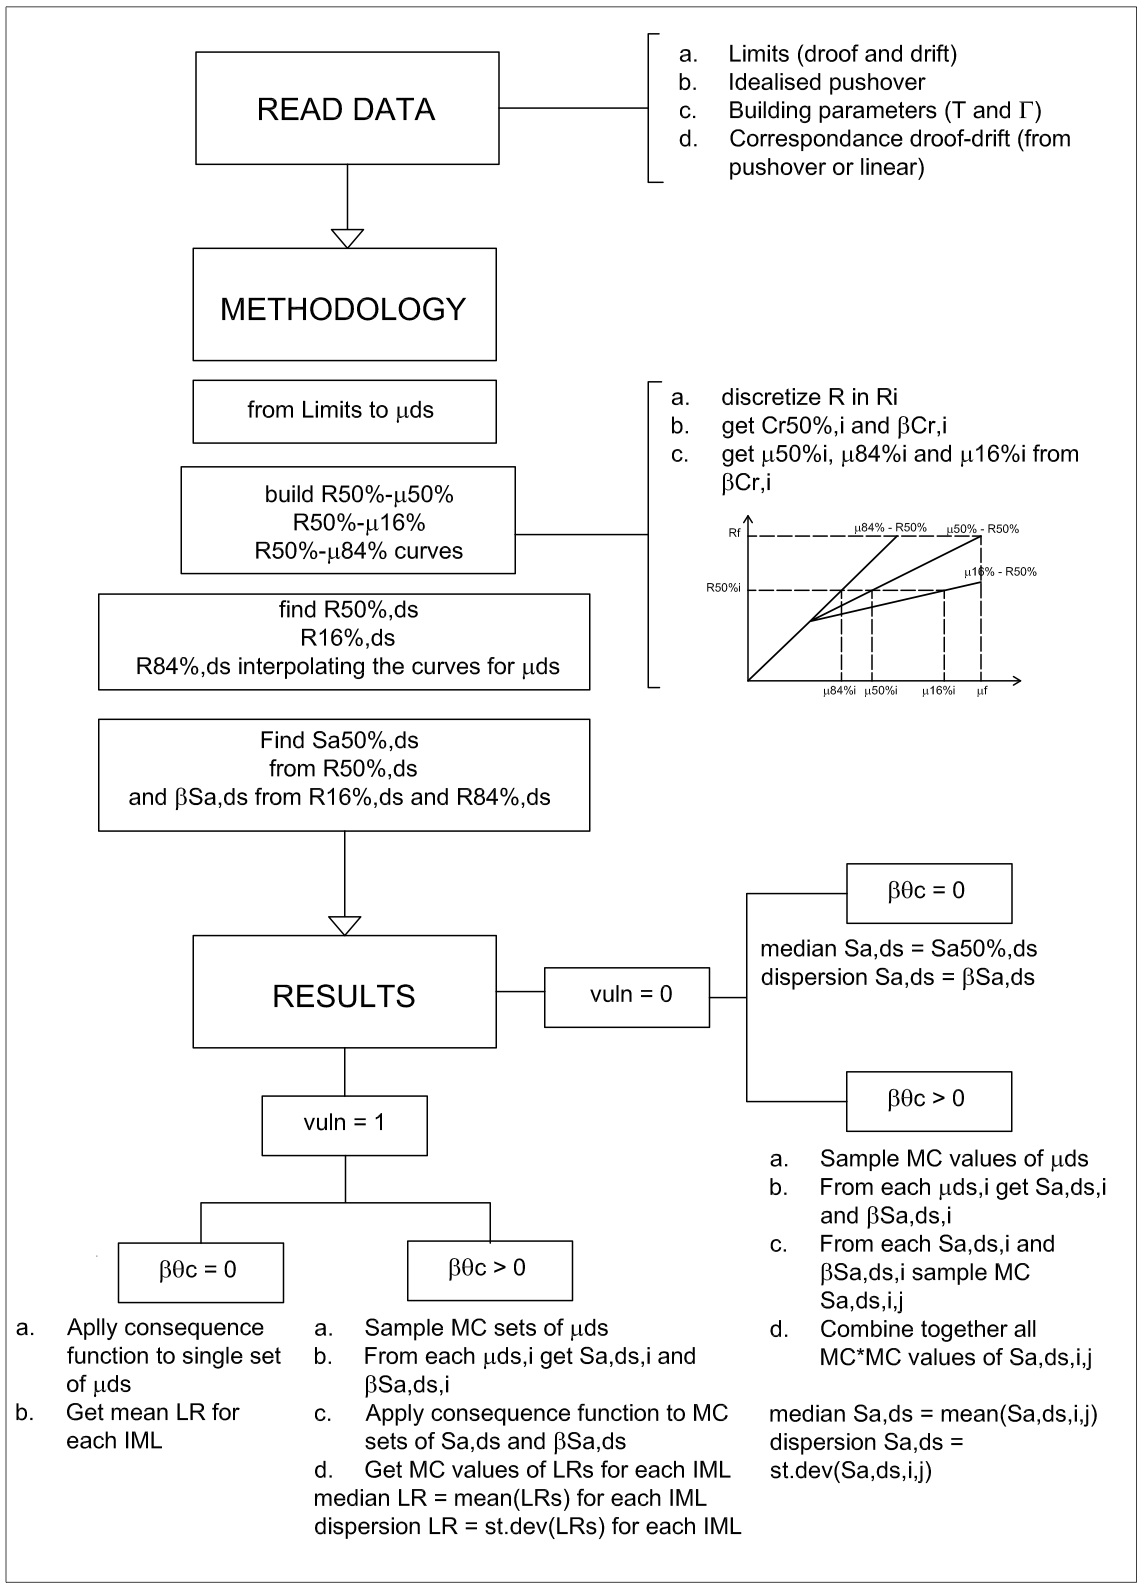
\includegraphics[width=15cm]{./figures/Cr-WorkFlow.jpg}
\caption{C$_R$-based procedure workflow.}
\label{fig:Cr_workflow}
\end{figure}

The option \textit{an\_type} must be set equal to 0 and the option \textit{in\_type} according to the input at disposal. The corresponding inputs should follow the requirements described in section \ref{subsubsec:InputCr}. Given this options the code proceeds with the following steps:\\

\begin{enumerate}
\item \textbf{Process Inputs within \textit{read\_data}  function}\\
\begin{enumerate}
\item If \textit{in\_type} = 0 roof displacement at limit states and idealised pushover are read from \textit{displacement\_profile.csv} and \textit{idealised\_curve.csv} respectively. A one-to-one relationship between roof displacement and drift is assumed.
\item If \textit{in\_type} = 1 results from pushover analysis are extracted from \textit{displacements\_pushover.csv} and \textit{reactions\_pushover.csv}, and drift limit states from \textit{limits.csv}. The relationship between drift and roof displacement is given by the pushover inputs.\\
The idealised 	pushover curve is then derived in the \textit{idealisation} function, where the idealisation process is conducted according to FEMA-440. The elastic stiffness is defined as the 	tangent stiffness passing through the point of the pushover curve where 60\% of the maximum base shear is reached, and the perfectly plastic branch is set at an height equal to 	the maximum base shear. The yielding point is found as the interception between the elastic and the plastic branch.\\
\end{enumerate}

Period, modal participation factor, number of buildings constituting the building class, importance factor (weight) of the each building within the class, average period of the class and $S_a(T_{av})/S_a(T_{blg})$ ratio are also returned by the function \textit{read\_data} .\\

\item \textbf{Fragility curve methodology}\\
The parameters extracted are used in the \textit{simplified\_bilinear} function, within the \textit{fragility\_process} function, to derive ductility levels $\mu_{ds}$, median spectral acceleration $\hat{S}_{a,ds}$ and the total dispersion $\beta_{S_a}$ at each limit state through the following steps:

\begin{enumerate}

\item The idealised MDoF system is transformed into an equivalent SDoF system, using $\Gamma_1$.

\item Ductility levels $\mu_{ds}$ corresponding to each damage threshold, are defined.

\item $\mu_{50\%}$ - $R_{50\%}$, $\mu_{16\%}$ - $R_{50\%}$ and $\mu_{84\%}$ - $R_{50\%}$ relationships are computed, as described in \ref{subsubsec:single-building}.

\item $R_{50\%}$ is computed for the ductility limit states $\mu_{ds}$, interpolating the aforementioned curves, and C$_{R_{50\%}}$ is calculated by mean of equation \ref{eq:Cr_RGM}.

\item $\hat{S}_{a,ds}$ and the corresponding dispersion $\beta_{S_{a d}}$ due to record-to-record variability are computed using eq. \ref{eq:SaR} and \ref{eq:betaR} for each limit state.

\item If dispersion due to uncertainty in the limit state $\beta_{\theta c}$ is different from zero, different ductility limit states are sampled for each median ductility level $\mu_{ds}$. For each sampled ductilities the corresponding $\hat{S}_{a,ds}$ and $\beta_{S_{a d}}$ are found as described in steps (d) and (e), and MC random S$_a$ for each of the MC sampled ductility limit states are computed using $\hat{S}_{a,ds}$ and $\beta_{S_{a d}}$.\\

\end{enumerate}

\item \textbf{Fragility curve results}\\
If number of buildings = 1\\
\begin{enumerate}
\item If \textit{vuln} = 0
the final values of median and dispersion of the fragility curves, $\hat{S}_{a,ds}$ and $\beta_{S_a}$, are computed as the mean and the standard deviation of the MC$^2$ samples of S$_a$, if many $\mu_{ds}$ were sampled at step 2.f, otherwise they correspond to the $\hat{S}_{a,ds}$ and $\beta_{S_{a d}}$, including only record-to-record variability, obtained at step 2.e.
All median values of S$_{a, ds}$ are converted to mean values $\mu_{ln(S_{a, ds})}$; mean $\mu_{ln(S_{a})}$ and total dispersion $\beta_{S_a}$ are then converted to logarithmic mean $\mu_{S_a}$ and logarithmic covariance $cov_{S_a}$, according to equations \ref{eq:median-to-mean} and \ref{eq:dispersion-to-standard} respectively.
Fragility curves for the building are displayed if the variable \textit{plotflag}[2] = 1, and logarithmic $\mu_{S_a}$ and $cov_{S_a}$ are exported in the \textit{outputs} folder.

\item 
If \textit{vuln} =1 if many values were sampled to account for uncertainty in the damage criteria at step 2.f, MC values of loss ratio LRs are defined for the MC sets of $\mu_{ds}$, using the \textit{damage\_to\_loss} function, for each intensity measure level defined in the variable \textit{iml} . Mean and standard deviation of LRs(iml), $\mu_{LR}$ and $\beta_{LR}$, are computed. If $\beta_{\theta c}$= 0 a single set of $\mu_{ds}$ is considered, resulting in no uncertainty in the LR for each iml.
Vulnerability curve for the building is displayed if the variable \textit{plotflag}[3] = 1, and $\mu_{LR}$ and $cov_{LR}$ at each iml are exported in the \textit{outputs} folder.\\

\end{enumerate}

If number of buildings > 1\\
\begin{enumerate}
\item If \textit{vuln} = 0
the final values of median and dispersion of the fragility curves, $\hat{S}_{a,ds}$ and $\beta_{S_a}$, are computed as the mean and the standard deviation of the MC$^2$ samples of S$_a$, if many $\mu_{ds}$ were sampled at step 2.f, otherwise they correspond to the $\hat{S}_{a,ds}$ and $\beta_{S_{a d}}$, including only record-to-record variability, obtained at step 2.e.

All $\hat{S}_{a, ds, blg}(T_1)$ are converted to mean values $\mu_{ln(S_{a, ds, blg})}(T_1)$ and then to the intensity measure in common with the rest of the buildings, $\mu_{ln(S_{a, ds, blg}(T_{av}))}$, according to eq. \ref{eq:Sa(Tav)}.\\
The $\mu_{ln(S_{a, ds, blg}(T_{av}))}$ are finally combined in a single lognormal curve for the building class, as described in section \ref{subsubsec:multiple-buildings}. 

Mean $\mu_{ln(S_{a})}$ and total dispersion $\beta_{S_a}$ are then converted to logarithmic mean $\mu_{S_a}$ and logarithmic covariance $cov_{S_a}$, according to equations \ref{eq:median-to-mean} and \ref{eq:dispersion-to-standard} respectively.

Fragility curves for the class of buildings are displayed if the variable \textit{plotflag}[2] = 1, and logarithmic $\mu_{S_a}$ and $cov_{S_a}$ are exported in the \textit{outputs} folder.

\item 
If \textit{vuln} =1
all $\hat{S}_{a, ds}(T_1)$ for each building are converted to mean $\mu_{ln(S_{a, ds})}(T_1)$ and then to the intensity measure in common with the rest of the buildings, $\mu_{ln(S_{a, ds, blg}(T_{av}))}$, according to eq. \ref{eq:Sa(Tav)}.

if many values were sampled to account for uncertainty in the damage criteria at step 2.f, MC values of loss ratio LRs are defined for the MC sets of $\mu_{ds}$, using the \textit{damage\_to\_loss} function, for each intensity measure level defined in the variable \textit{iml}. Mean and standard deviation of LRs(iml), $\mu_{LR}$ and $\beta_{LR}$, are computed. If $\beta_{\theta c}$= 0 a single set of $\mu_{ds}$ is considered, resulting in no uncertainty in the LR for each iml.
The $\mu_{LR, iml, blg}$ are finally combined in a single mean and standard deviations, as described in section \ref{subsubsec:multiple-buildings}. Vulnerability curve for the class of buildings is displayed if the variable \textit{plotflag}[3] = 1, and $\mu_{LR}$ and $cov_{LR}$ at each iml are exported in the \textit{outputs} folder.

\end{enumerate}

\end{enumerate}
